\section{Simulations Experiments}
\label{sec:simulationexperiments}


This section presents the experimental results of the simulations of our proposed \ac{REACT} method. The entire framework is implemented in C++ to ensure computational efficiency and is integrated with ROS to facilitate modularity and deployment on real-world robots. Furthermore, the \ac{OMPL} library \cite{ompl} was utilized to compute the shortest paths using the RRT* algorithm.  


\subsection{Simulation experimental setup }
The path planner is implemented for a BlueROV2. A \ac{MPC} approach is used to account for model constraints and provide the optimal control input $\mathbf{u}^{ref} \in \mathbb{R}^4$, where $\mathbf{u}^{ref} = [F_x, F_y, F_z, M_z]^T$ represents the forces in the $X$, $Y$, and $Z$ directions, and the moment about the $Z$-axis. The goal is to follow the desired reference trajectory $\mathbf{x}^{ref} \in \mathbb{R}^6$, where $\mathbf{x}^{ref} = [x_{ref}, y_{ref}, z_{ref}, \psi_{ref}]^T$ contains the reference position ($x_{ref}$, $y_{ref}$, $z_{ref}$) and the reference yaw angle $\psi_{ref}$.

The entanglement-aware path planner provides $\mathbf{x}^{ref}$ in real time, ensuring the BlueROV2 avoids obstacles while following the desired trajectory. For further details about the controller and model, the reader is referred to \cite{amergp}.

%\subsection{Results}
We perform a comparative analysis of the proposed \ac{REACT} method and a baseline conventional \ac{CPP} (FC-Planner \cite{feng2024fc}), which does not contain explicit handling of entanglement. 

The simulation setup consists of a pipe structure represented by an underwater pipe model from \cite{feng2024fc}. The simulated onboard camera featured a field of view of 70 degrees. The tether constraint was defined by a maximum allowed tether length of $L_{max}$ = 10.0 meters.

Environmental coverage was evaluated geometrically similar to \cite{amer2023visual}. At each subsampled time step, the position and orientation of the camera were used to determine which triangles in the environment mesh were visible. A triangle was marked as visible if its centroid was within the inspection range, its surface normal faced the camera, and its projection lay within the camera's field of view. Over time, the set of all uniquely observed triangles was accumulated. The coverage at time $t$ was defined as the ratio of the number of unique visible triangles up to time $t$ to the total number of triangles in the environment.


\subsection{Simulations results}

%The quantitative performance metrics for both planners are summarized in Table~\ref{tab:performance_metrics}. Figures~\ref{fig:coverage_vs_time} and~\ref{fig:tether_vs_time} visualize the performance of the planners in terms of environmental coverage and tether length, respectively.







\begin{table}[t]
    \centering
    \caption{Coverage performance comparison between \ac{REACT} and \ac{CPP} baseline showing inspection time, recovery time, total mission duration, and final environmental coverage. }

    \label{tab:performance_metrics}
    {\large
    \resizebox{1.0\columnwidth}{!}{%
    \begin{tabular}{|l|c|c|c|c|}
        \hline
        \textbf{Planner} & \textbf{Inspection time (s)} & \textbf{Recovery time (s)} & \textbf{Total time (s)} & \textbf{Coverage (\%)} \\
        \hline
        \ac{REACT} & 546 & 134 & \textbf{680} & \textbf{99.91} \\
        CPP & 429 & 426 & 855 & 99.82 \\
        \hline
    \end{tabular}%
    }
    }
    \vspace{0.5em}
\end{table}


\begin{table}[b]
    \centering
    \caption{Comparison of tether constraint compliance showing the maximum tether length reached and the total duration of tether length exceedance.}
    \label{tab:tether_metrics}
    {\Large
    \resizebox{1.0\columnwidth}{!}{%
    \begin{tabular}{|l|c|c|}
        \hline
        \textbf{Planner} & \textbf{Maximum tether length (m)} & \textbf{Duration of length exceedance (s)} \\
        \hline
        CPP & 31.16 & 327.37 \\
        \ac{REACT} & \textbf{10.52} & \textbf{10.36} \\
        \hline
    \end{tabular}%
    }
    }
    \vspace{0.5em}
\end{table}









\begin{figure}[t]
    \centering
    \begin{subfigure}[b]{0.48\linewidth}
        \centering
        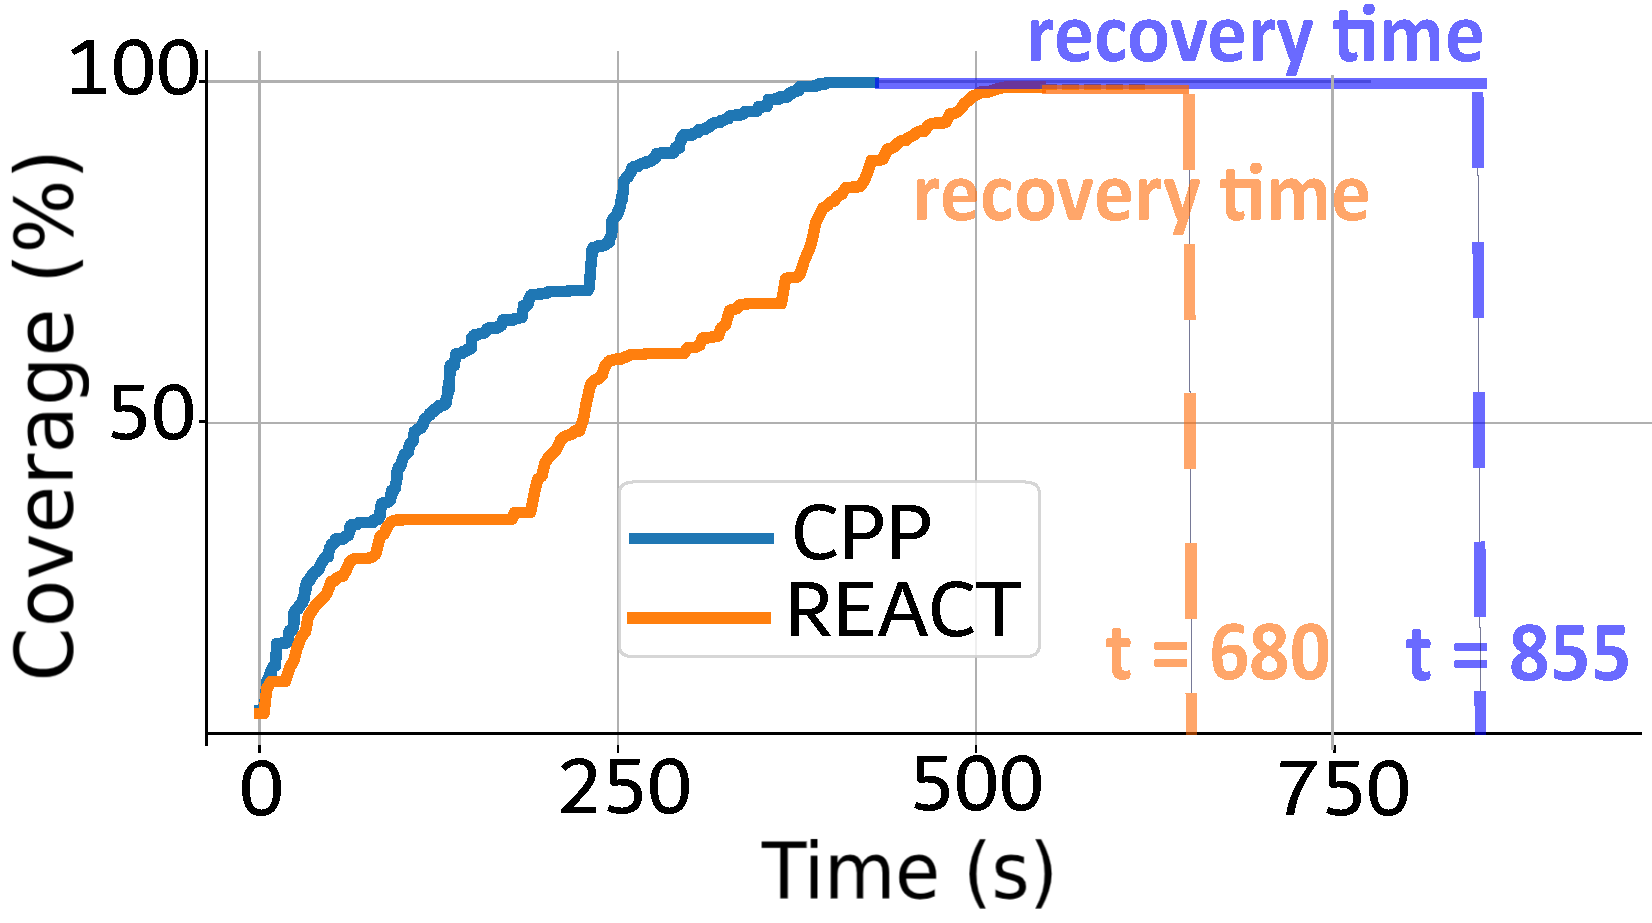
\includegraphics[width=\linewidth]
        {coverage_vs_time_recovery.pdf}
        %{coverage_vs_time.pdf}
        \caption{ Coverage vs. Time.}
        \label{fig:coverage_vs_time}
    \end{subfigure}
    \hfill
    \begin{subfigure}[b]{0.48\linewidth}
        \centering
        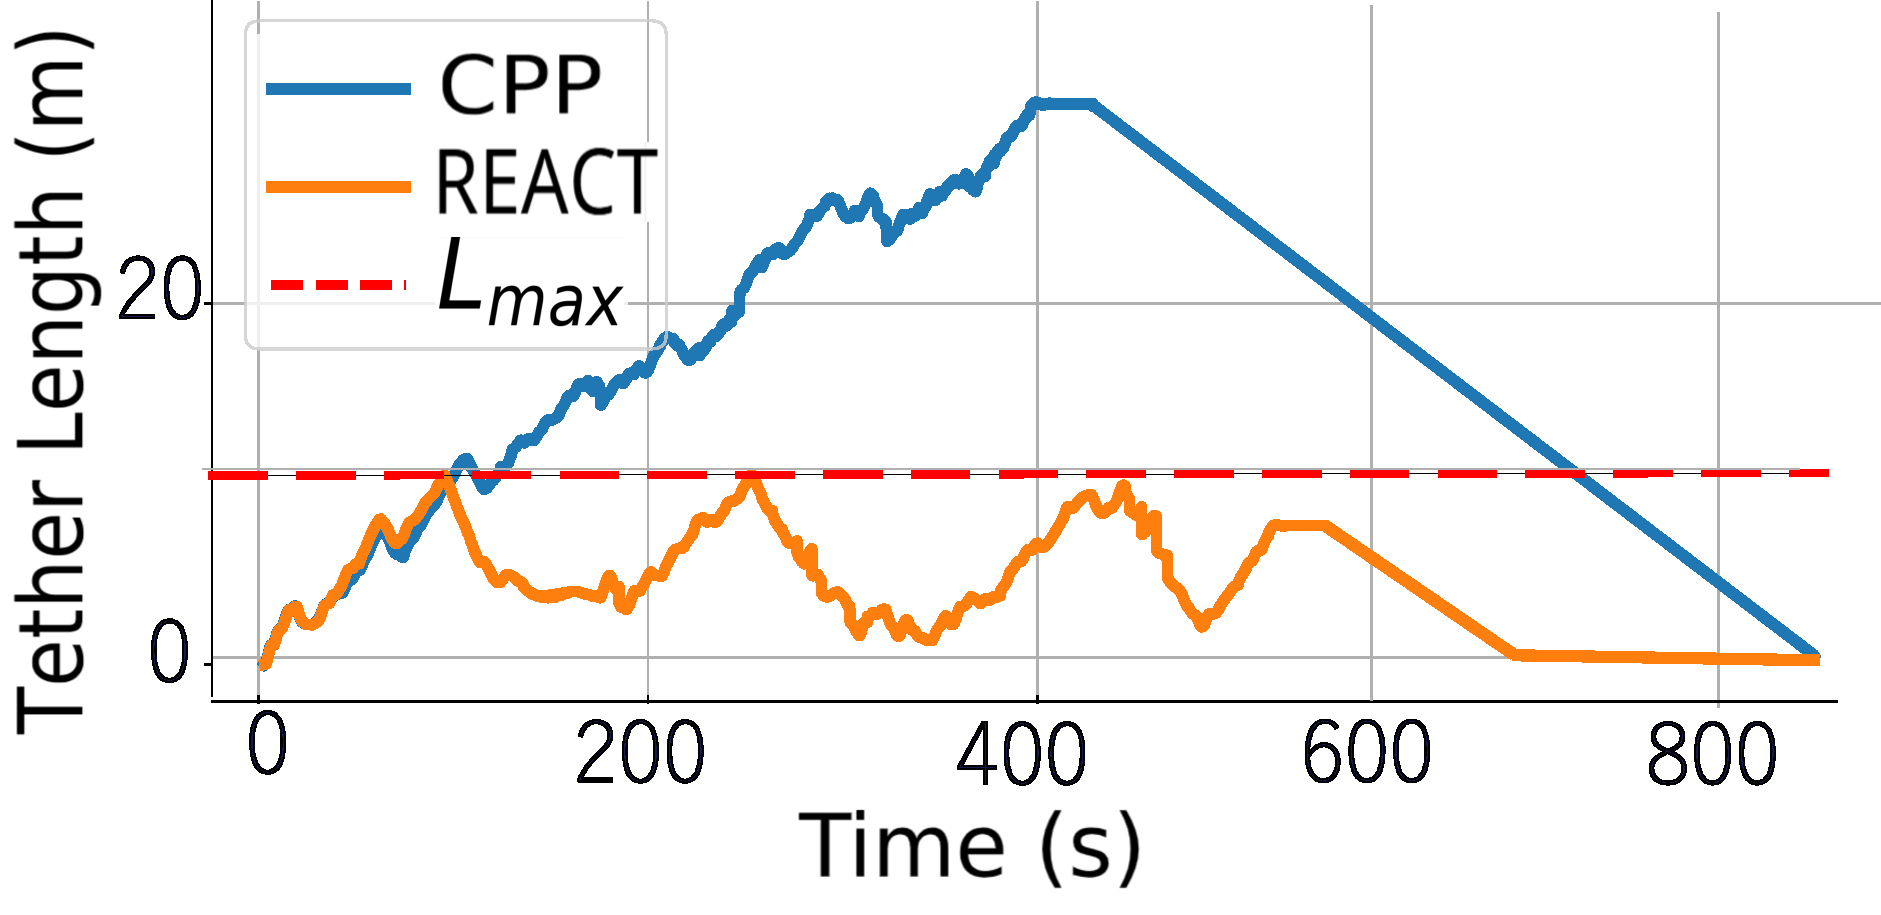
\includegraphics[width=\linewidth]{EA-Planner/figures/tether_length_vs_time_with_recovery.pdf}
        \caption{Tether Length vs. Time.}
        \label{fig:tether_vs_time}
    \end{subfigure}
    \caption{Comparison of coverage and tether behavior over time.}
    \label{fig:coverage_tether_sidebyside}
\end{figure}


\begin{figure}[ht]
    \centering
    \begin{subfigure}[b]{0.48\linewidth}
        \centering
        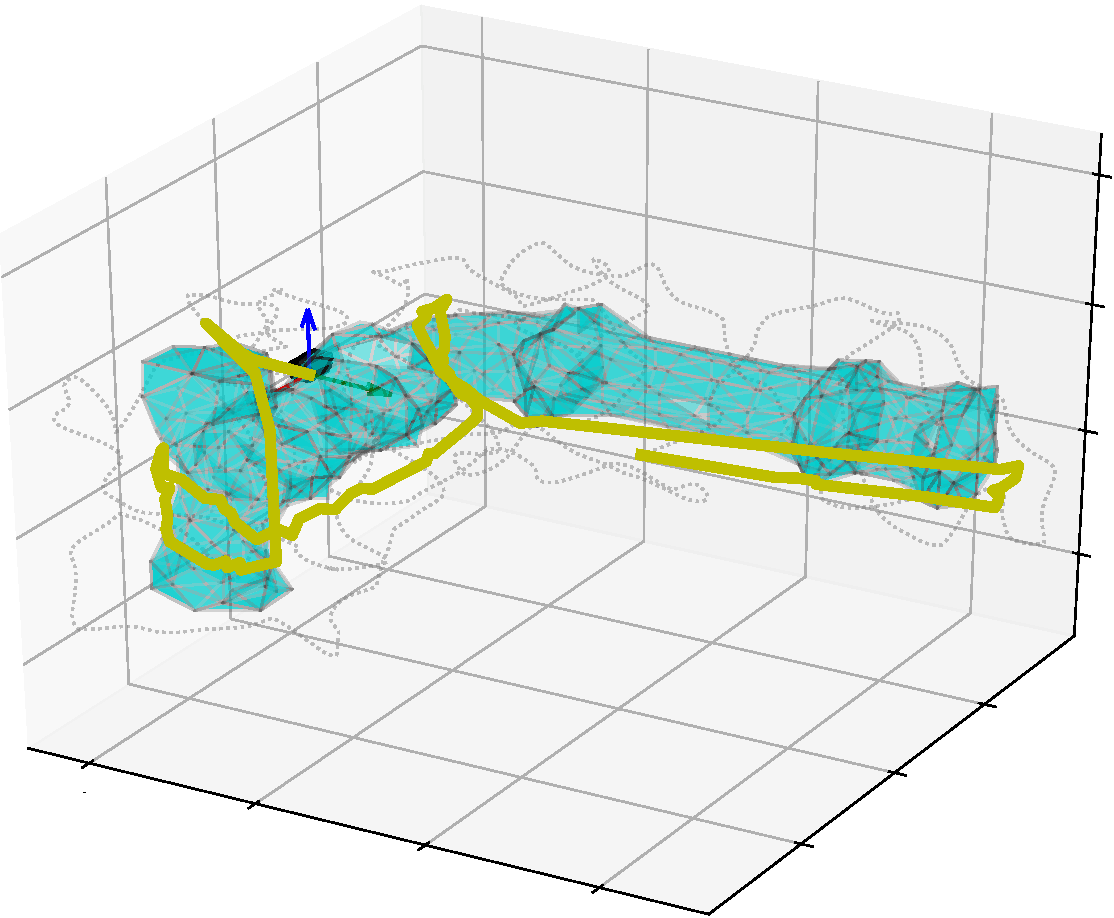
\includegraphics[width=\linewidth]{EA-Planner/figures/fc_planner_final_view.pdf}
        \caption{\ac{CPP} final tether path.}
        \label{fig:3d_cpp}
    \end{subfigure}
    \hfill
    \begin{subfigure}[b]{0.48\linewidth}
        \centering
        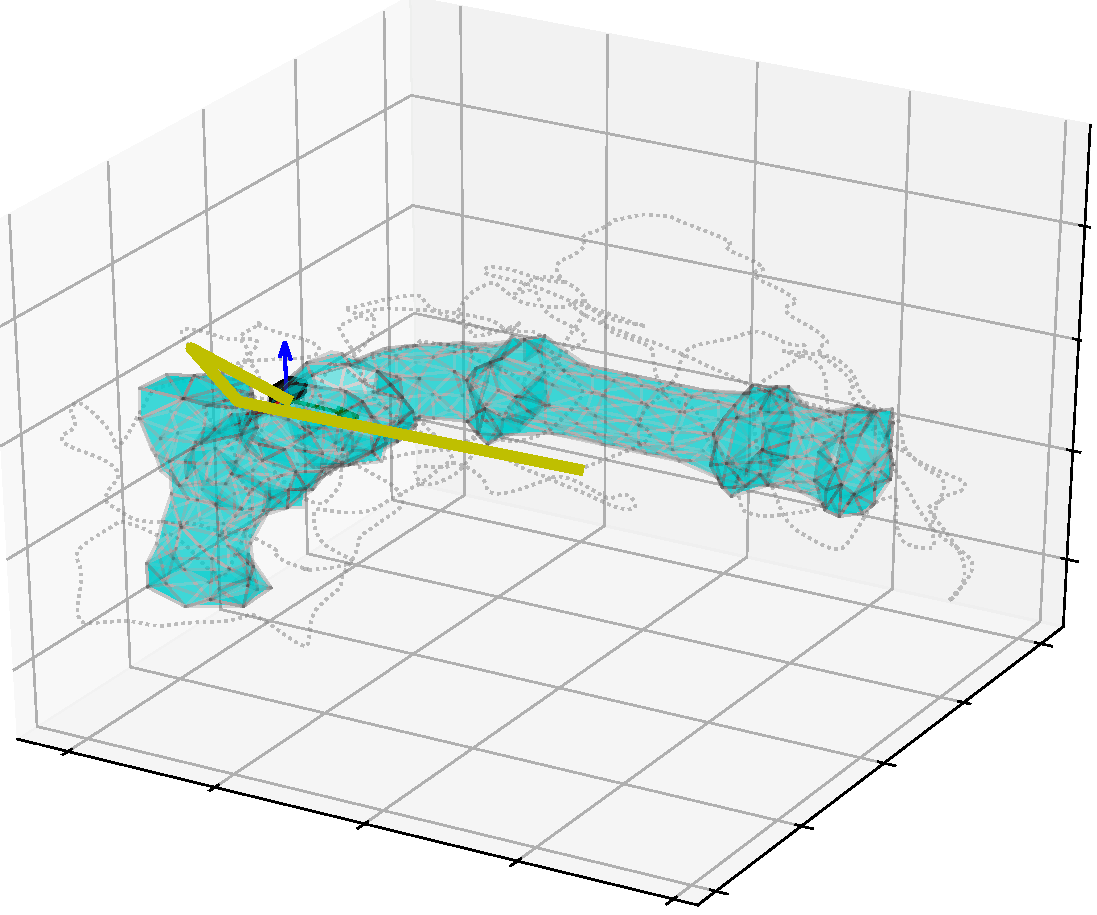
\includegraphics[width=\linewidth]{EA-Planner/figures/react_pipe.pdf}
        \caption{\ac{REACT} final tether path.}
        \label{fig:3d_oea}
    \end{subfigure}
    \caption{3D views of final trajectories. (a) CPP results in entangled tether path. (b) \ac{REACT} yields a non-entangled tether path, reflecting effective entanglement avoidance.}
    \label{fig:3Dplots}
\end{figure}
% The results highlight distinct trade-offs between the two planning strategies. The \ac{CPP}, lacking entanglement awareness, completed the trajectory significantly faster (429.00~s vs. 546.00~s) while achieving marginally less final coverage (99.81\% vs. 99.91\%). However, focusing solely on speed and final coverage overlooks the critical aspect of tether management in constrained environments. As shown in Figure~\ref{fig:tether_vs_time},\ac{CPP} planner exceeded the $L_{\text{max}}$ constraint during execution. 

% \ac{REACT} is explicitly designed to avoid and respond to potential tether entanglement. Its reactive replanning untangles the tether from entangled configurations. 

% Conversely, the \ac{CPP}, lacking entanglement- awareness, proceeds along its path violating the maximum tether length constraint. While this happened slightly later in this simulation, the approach risks encountering more severe or unrecoverable tether states without the ability to proactively mitigate them.

% The longer execution time of the \ac{REACT} directly is a result of executing reactive replanning maneuvers when necessary. This deliberate approach prioritizes tether safety and mission robustness over raw speed, offering a significant advantage for reliable operation in complex, real-world underwater scenarios where tether integrity is paramount. 

% The \ac{CPP}'s coverage speed advantage comes at the cost of ignoring potential tether hazards, making it less suitable for missions where entanglement poses a significant risk. Therefore, \ac{REACT} demonstrates superior performance in the context of safe and robust tethered \ac{ROV} operation, despite the longer completion time observed in this comparison.


The performance metrics for both planners are summarized in Table~\ref{tab:performance_metrics} and Table~\ref{tab:tether_metrics}, while Figures~\ref{fig:coverage_tether_sidebyside} and~\ref{fig:3Dplots} visualize the performance of the planners in terms of environmental coverage, tether length behavior, and final trajectory configurations. The evaluation focuses on comparing mission efficiency, constraint compliance, and safety aspects between the entanglement-aware \ac{REACT} method and the conventional \ac{CPP} baseline approach.



%The simulation experimental results demonstrate the effectiveness of our proposed \ac{REACT} method, which  continuously evaluates the tether path through the maximum tether length constraint. When \ac{REACT} detects potential entanglement or constraint violation, it dynamically finds alternative paths that disentangle the \ac{ROV} and then redirects toward the original waypoint. 

The results are presented in two phases: the inspection phase and the recovery phase, where the recovery time represents the estimated duration required to return to the starting position after complete inspection while disentangling the entire tether.

The results highlight distinct trade-offs between the two planning strategies. As shown in Table~\ref{tab:performance_metrics}, the \ac{CPP} method achieves a shorter inspection time (429s vs. 546s) due to its straightforward path execution without rerouting for disentanglement. However, focusing solely on inspection speed overlooks the critical aspect of tether management in constrained environments. The \ac{CPP} exhibits a significantly longer total mission time (855s vs. 680s) because extensive disentanglement is required after inspection completion.

The \ac{REACT} method demonstrates multiple instances of detection and resolution of entanglement, evidenced by the peaks in the tether length curve in Figure~\ref{fig:tether_vs_time} and the corresponding flat regions in the coverage curve in Figure~\ref{fig:coverage_vs_time}, where the \ac{ROV} inspection progress is stopped to reroute and find entanglement-free paths. This reactive replanning behavior directly results in the longer inspection time, as the system prioritizes tether safety over raw speed.

Notably, the tether length constraint is rarely exceeded by \ac{REACT} (maximum 10.52m vs. constraint of 10.0m), as shown in Table~\ref{tab:tether_metrics}. Conversely, the \ac{CPP} method severely violates this constraint, reaching 31.16m for extended periods (327.37s), risking unrecoverable tether states without the ability to proactively mitigate them. The 3D trajectory visualizations in Figure~\ref{fig:3Dplots} further illustrate this difference, showing the entangled tether geometry resulting from \ac{CPP} versus the non-entangled configuration achieved by \ac{REACT}. Therefore, \ac{REACT} demonstrates superior performance for safe tethered \ac{ROV} inspection.

